\chapter{在你感觉准备好之前采取行动}\label{chap:w5}

\noindent \href{https://github.com/taseikyo/arts}{readme} | \hyperref[chap:w4]{previous} | \hyperref[chap:w6]{next}

\begin{figure}[htbp]
  \centering
    
\includegraphics[width=\textwidth]{../images/2020/12/claudio-schwarz-purzlbaum-Zh-btVpBcdw-unsplash.jpg}
  \caption{\textit{Photo by 🇨🇭 Claudio Schwarz | @purzlbaum on Unsplash}}
\end{figure}


\textit{总字数:3394 个(汉字:2235,英文单词:396,数字:134,中文标点:270,英文标点:359),阅读时长约:6 分 40 秒。}

\section{algorithm \hyperref[chap:w5]{top}}\label{w5:algorithm}

\subsection{\href{https://leetcode-cn.com/problems/count-complete-tree-nodes/}{222.完全二叉树的节点个数}}

给出一个完全二叉树,求出该树的节点个数。

直接递归挺简单的:

\begin{lstlisting}[language=go]
func countNodes(root *TreeNode) int {
	if root == nil {
		return 0
	}
	return 1 + countNodes(root.Left) + countNodes(root.Right);
}
\end{lstlisting}

官方题解给出了一个二分查找+位运算的解法,好是好,但是面试的时候肯定想不出来:

规定根节点位于第 0 层,完全二叉树的最大层数为 h。

如果第 k 个节点位于第 h 层,则 k 的二进制表示包含 h+1 位,其中最高位是 1,其余各位从高到低表示从根节点到第 k 个节点的路径,0 表示移动到左子节点,1 表示移动到右子节点。通过位运算得到第 k 个节点对应的路径,判断该路径对应的节点是否存在,即可判断第 k 个节点是否存在。

如果第 k 个节点存在,则节点个数一定大于或等于 k,如果第 k 个节点不存在,则节点个数一定小于 k,由此可以将查找的范围缩小一半,直到得到节点个数。

\begin{figure}[htbp]
  \centering
    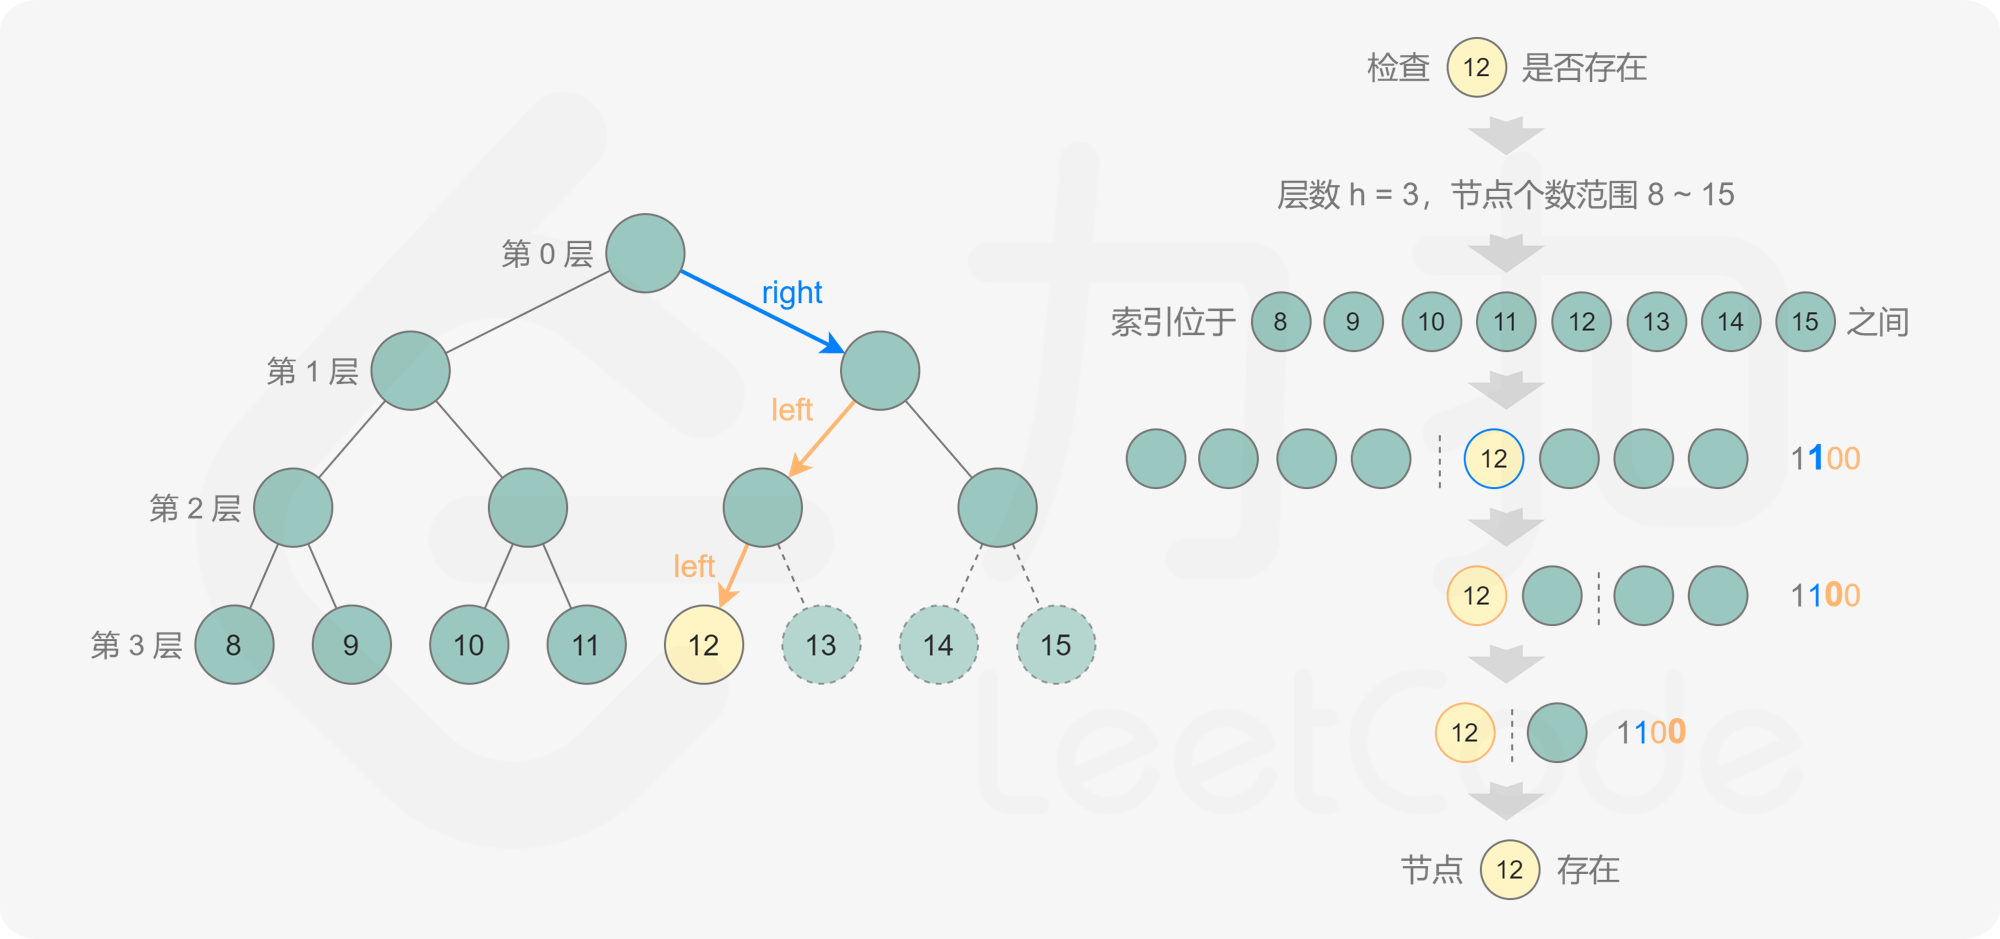
\includegraphics[width=\textwidth]{../images/2020/12/w5-algo-1.png}
  \caption{\textit{w5-algo-1.png}}
\end{figure}

\begin{myquote}
\textcolor{gray}{注:sort 包中的 func Search(n int, f func(int) bool) int 解释}
\end{myquote}

\begin{myquote}
\textcolor{gray}{Search 采用二分法搜索找到 [0, n) 区间内最小的满足 f(i)==true 的值 i}
\end{myquote}

\begin{lstlisting}[language=go]
func countNodes(root *TreeNode) int {
	if root == nil {
		return 0
	}
	level := 0
	for node := root; node.Left != nil; node = node.Left {
		level++
	}
	return sort.Search(1<<(level+1), func(k int) bool {
		if k <= 1<<level {
			return false
		}
		bits := 1 << (level - 1)
		node := root
		for node != nil && bits > 0 {
			if bits&k == 0 {
				node = node.Left
			} else {
				node = node.Right
			}
			bits >>= 1
		}
		return node == nil
	}) - 1
}
\end{lstlisting}

\section{review \hyperref[chap:w5]{top}}\label{w5:review}

\subsection{\href{https://nibblestew.blogspot.com/2020/11/the-nine-phases-of-open-source-project.html}{开源项目维护者的九个阶段(英文)}}

作者提出开源项目维护者经历的两个时期(stage)九个阶段(phase),第一个时期包括五个阶段,第二个时期包括四个阶段:

\begin{itemize}
\item The Project Is Mostly for Yourself
  \begin{enumerate}
    \item The Inventor(发明者)
    \item The MVP Implementer(实现者)
    \item The Ditch Digger(挖掘机(大雾))
    \item The Documentation Writer(文档写手)
    \item The Marketer(营销人员)
  \end{enumerate}
\item The Project Is Mostly for Other People
\end{itemize}

看着这九个阶段,我觉得跟一个人创业到发展壮大再到退休类似。

开始作为个人开发者,有个好点子,出于兴趣或是其他原因将其实现并开源,为了让其他人使用或者是加入开发我们需要为其写 README,操作手册之类的文档,之后为了进一步壮大需要一个营销推手,整一个热搜推广一波,让更多人了解和使用。

当项目成熟壮大之后,就需要招募更多人手,然后你作为创始人就会退出开发的一线,成为一个标准的制定者和维护者,实际的开发工作交给新来的人,你做一下决策即可。再往后,你退出开发,甚至决策,这个时候,这个项目要么已经被废弃,要么变成另一个项目,但是此时都与你当初那个项目完全不同了,或许你会作为一个创始者与这个项目一起被记住。

我作为一个开源项目开发者(算是吧)现在尽量养成一个写好文档和注释的习惯,因为让别人去看代码来了解功能的项目是一个垃圾项目,作为开发者,我可能仅仅只是想使用你的某些 API,我不想看你的代码,不想管你的实现细节,直接告诉我怎么使用就好了。

另外作为开源项目维护者,出于兴趣也好,出于充实自己简历的目的也好,如果想维护好这个项目,它是没有终点的,你需要一直坚持维护更新,半途而废的项目是没意义的,浪费了自己的时间和精力(如第二期的主题:\href{https://github.com/taseikyo/arts/blob/master/weekly/202011w2.md}{忘记业余项目,专注于工作}),而且开源意味着基本没有收益,除非你做的非常好。正如作者所说,\textit{After all, a half dug ditch is about as useless as a completely undigged ditch. It's only when you reach the end and water starts flowing that you get any benefits. The difference between physical ditches and sotware is that there is no reliable way of estimating how much more you still have to dig. ...The difference between physical ditches and software is that there is no reliable way of estimating how much more you still have to dig.}

\section{tip \hyperref[chap:w5]{top}}\label{w5:tip}

\subsection{\href{https://learnku.com/articles/23411/the-difference-between-rune-and-byte-of-go}{go 的 [] rune 和 [] byte 区别(中文)}}

原文是英文,但是对应链接打不开了。

在 go 中,byte 占一个字节,类似 c 中的 char(go 没有 char 这个类型),而 rune 占四个字节,所以 \lstinline{[]rune(s)} \lstinline{[]byte(s)} 这俩有啥区别?

\begin{lstlisting}[language=go]
first := "fisrt"
fmt.Println([]rune(first))
fmt.Println([]byte(first))
\end{lstlisting}

\begin{myquote}
\textcolor{gray}{[102 105 115 114 116] // 输出结果 [] rune}
\end{myquote}

\begin{myquote}
\textcolor{gray}{[102 105 115 114 116] // 输出结果 [] byte}
\end{myquote}

由于字母根据 ASCII 编码都是一个字节,看不出什么,下面中文就可以看出区别了。

\begin{lstlisting}[language=go]
first := "社区"
fmt.Println([]rune(first))
fmt.Println([]byte(first))
\end{lstlisting}

\begin{myquote}
\textcolor{gray}{[31038 21306] // 输出结果 [] rune}
\end{myquote}

\begin{myquote}
\textcolor{gray}{[231 164 190 229 140 186]// 输出结果 [] byte}
\end{myquote}

\begin{lstlisting}[language=go]
s := "截取中文"
//试试这样能不能截取?
fmt.Println(s[:2])
\end{lstlisting}

\begin{myquote}
\textcolor{gray}{?? // 输出 在预料之中, 输出了常见的??}
\end{myquote}

\begin{lstlisting}[language=go]
s := "截取中文"
//试试这样能不能截取?
res := []rune(s)
fmt.Println(string(res[:2]))
\end{lstlisting}

\begin{myquote}
\textcolor{gray}{截取 // 输出,顺利截取了}
\end{myquote}

当你直接使用 \lstinline{s[:2]} 进行截取的时候,底层会将中文转化成 \lstinline{[]byte}, 而不是 \lstinline{[]rune},当我尝试 \lstinline{fmt.Println(s[:3])} 的时候正常打印出 "截"。

\subsection{\href{https://baijiahao.baidu.com/s?id=1659926342373074716}{Win10 无敌输入法诞生:微软拼音+搜狗词库(中文)}}

在苦恼于微软自带输入法瘠薄的词库时发现了这篇文章,主要就是使用 \href{https://github.com/studyzy/imewlconverter}{studyzy/imewlconverter} 这个转换工具,将下载好的搜狗词库转化为微软输入法的\textbf{自学词汇}或者\textbf{自定义短语},由于自学词汇有长度限制,而自定义短语没有,当词库过大时可以转短语,但是导入大量短语后设置界面会卡住(别问我怎么知道的),所以感觉还是自学词库好一点,然鹅有长度限制,各有利弊吧。

另外还学到了一个技巧:\textbf{英文提示}。微软输入法只有在中文输入时,才会有英文单词提示,但是使用效果并不是很理想,可能输了好多字母才开始提示,而且提示的那个单词并不是我想要的。

这个好用的技巧是在输入第一个字母时按住 shift,也就是第一个字母大写,然后就转为一种类似英文的提示输入了,虽然每次需要把第一个字母改回小写,但是英文提示功能大大增强了,算是一个不错的技巧了。

\subsection{\href{https://www.imooc.com/wenda/detail/578468}{Windows 上是否有 \lstinline{/dev/null}?(中文)}}

\begin{myquote}
@慕容4345310:我想你想要NUL,至少在命令提示符或批处理文件中。
\end{myquote}

\begin{myquote}
例如:
\end{myquote}

\begin{myquote}
type c:\textbackslash autoexec.bat > NUL
\end{myquote}

\begin{myquote}
不创建文件。(我相信如果您尝试以编程方式创建文件也是如此,但我还没有尝试过。)
\end{myquote}

\begin{myquote}
在 PowerShell 中,您需要 \$null:
\end{myquote}

\begin{myquote}
echo 1 > \$null
\end{myquote}

\begin{myquote}
@德玛西亚99:NUL 在 Windows 中似乎实际上是任何文件夹中的虚拟路径。就像..,.在任何文件系统。
\end{myquote}

\begin{myquote}
使用NUL后面的任何文件夹都可以。
\end{myquote}

\begin{myquote}
例,
\end{myquote}

\begin{myquote}
echo 1 > nul
\end{myquote}

\begin{myquote}
echo 1 > c:\textbackslash nul
\end{myquote}

\begin{myquote}
echo 1 > c:\textbackslash users\textbackslash nul
\end{myquote}

\begin{myquote}
echo 1 > c:\textbackslash windows\textbackslash nul
\end{myquote}

\begin{myquote}
与/dev/nullLinux上的效果相同。
\end{myquote}

\begin{myquote}
这是在 Windows 7,64 位上测试的。
\end{myquote}

\section{share \hyperref[chap:w5]{top}}\label{w5:share}

\subsection{\href{https://medium.com/the-ascent/why-you-should-take-action-before-you-feel-ready-not-after-16e41e5b840f}{在你感觉准备好之前采取行动(英文)}}

\textit{There's no way life is going to get better on its own. You have to make it better and the only way to do that is to act now, despite any resistance. (生活不可能自己变得更好。你必须让它变得更好,唯一的办法就是不顾任何阻力,现在就采取行动。)}

作者想表达的观点大概就是勇敢地采取行动,不要等到你自己“感觉”准备好了才开始,那样的话可能是年复一年的持续荒废时间。但是真的做到这一点并不简单,中国人讲究万事俱备,等所有准备工作就绪之后再开始,可能这是中西方的思维差异,西方人可能更“放肆”、更大胆,所以他们古有环球旅行,今有横穿亚马逊。当然随着全球文化交流的加深,中国人的思维也在渐渐改变,不是也有所谓的“说走就走的旅行”,“世界那么大,我想去看看”吗?(笑)。

扯远了,对我来说这算是一个权衡(trade-off)的问题,你是求稳还是更想尝试新事物?虽然在准备好之前采取行动确实能尝试更多新事物,带来的结果或好或坏(因为没有搞好准备工作,所以结果如何并不能确定),也许会一落千丈,骨头都不剩;也许会鸿运当头,从此人上人。

我啊,早早就认清自己,普普通通一个平凡人罢了,只想安稳过完一生,并不想尝试所谓的新事物,那些新奇、疯狂的想法看看/听听别人的事迹就够了,为什么会有人觉得没有做某件事人生就不完整?很喜欢鹿丸的一句话:\textit{我本来想过着随便当个忍者,随便赚点钱...然后和不美又不丑的女人结婚,生两个小孩,第一个是女孩,第二个是男孩...等长女儿结婚,儿子也能够独当一面的时候,就从忍者的工作退休...之后,每天过着下将棋或围棋的悠闲隐居生活...然后比自己的老婆还要早老死...我就是想过这种生活...}

\noindent \href{https://github.com/taseikyo/arts}{readme} | \hyperref[chap:w4]{previous} | \hyperref[chap:w6]{next}
